\documentclass{article}
\textheight 23.5cm \textwidth 15.8cm
%\leftskip -1cm
\topmargin -1.5cm \oddsidemargin 0.3cm \evensidemargin -0.3cm
%\documentclass[final]{siamltex}

\usepackage{verbatim}
\usepackage{fancyhdr}
\usepackage{amssymb,ctex}
\usepackage{mathrsfs}
\usepackage{latexsym,amsmath,amssymb,amsfonts,epsfig,graphicx,cite,psfrag}
\usepackage{eepic,color,colordvi,amscd}
\usepackage{enumerate}
\usepackage{booktabs}
\usepackage{graphicx}
\usepackage{float}
\usepackage{multirow}


\title{Numerical Analysis Homework9}
\author{Zhang Jiyao,PB20000204}

\begin{document}
	\maketitle
	
	\section{Introduction}
    
    \textbf{问题1}
    
    应用RKF45或RKF54方法,设计实现自适应方法,求解如下常微分方程初值问题:
    $$	
    \left\{ 
    \begin{array}{lc}
    	y' = e^{yx}+cos(y-x) \\
        y(1) = 3 \\
    \end{array}
    \right.$$
    
    初值步长取为$h=0.01$,在自适应方法中步长的选取采用第二种策略。
    
    在解溢出前终止,输出时输出解的范围;要求输入一个介于上述范围的值,应用简单的两点线性插值计算出对应的函数值。
    
    \textbf{问题2}
    
    初值问题 
     $$	
    \left\{ 
    \begin{array}{lc}
    	x' = \frac{t-e^{-t}}{x+e^x} \\
    	x(0) = 0 \\
    \end{array}
    \right.$$
    
    该方程的真解由等式
    $$ x^2-t^2+2e^x-2e^{-t}=0$$
    隐式给出。
    
    当$t=1$时,数值求解等式$x^2-t^2+2e^x-2e^{-t}=0$,将这一数值解作为参考的准确解。
    
    利用\text{Adams-Bashforth}公式计算方程在$t=1$的数值解,利用\text{Runge-Kunta}格式得到初值,取节点$x_i,i=0,...,N$,$N=2^k$,$k=3,...,8$,并给出误差表格。
	
	
	\section{Method}
	
	对于第一个问题,利用RKF54方法,我们有
	
	\begin{align*}
		y(x+h) &= y(x)+\sum_{i=1}^{6}a_iF_i \\
		&= y(x)+\frac{16}{135}F_1+\frac{6656}{12825}F_3+\frac{28561}{56430}F_4-\frac{9}{50}F_5+\frac{2}{55}F_6 \\
	\end{align*}

其中 

	\begin{align*}
	F_1 &= hf(x,y) \\
	F_2 &= hf(x+\frac{h}{4},y+\frac{F_1}{4})\\
	F_3 &= hf(x+\frac{3h}{8},y+\frac{3F_1}{32}+\frac{9F_2}{32})\\
	F_4 &= hf(x+\frac{12h}{13},y+\frac{1932F_1}{2197}-\frac{7200F_2}{2197}+\frac{7296F_3}{2197})\\
	F_5 &= hf(x+h,y+\frac{439F_1}{216}-8F_2+\frac{3680}{513}F_3-\frac{845F_4}{4104})\\
	F_6 &= hf(x+\frac{h}{2},y-\frac{8F_1}{27}+2F_2-\frac{3544}{2565}F_3+\frac{1859}{4104}F_4-\frac{11}{40}F_5)\\
   \end{align*}

  对于自适应算法选取步长,采用第二种策略:在每一步计算后,采用如下通用公式确定下一步的步长
  $$ h=0.9h(\frac{\delta}{|e|})^{\frac{1}{1+p}}  $$
  
  $p$是\text{Runge-Kutta}方法中第一个公式的阶。
  
  考虑局部截断误差:设$v$是在$x_0+h$上近似解的值,它是从$x_0$出发取长度为$h$的步长一步得到的;设$u$是在$x_0+h$上的另一种数值近似解,它是从$x_0$出发取长度为$\frac{h}{2}$步长进行两步计算得到的。$u,v$可以计算。
  
  局部截断误差为:
  $$  Ch^5=\frac{u-v}{1-2^{-4}} \approx u-v $$
  
  对于问题2:
  
  先利用五阶的\text{Runge-Kunta}公式得到$y_1,y_2,y_3,y_4$的值,然后启动公式,运用\text{Adams-Bashforth}公式
  $$ y_{n+1}=y_n+\frac{h}{720}(1901f_n-2774f_{n-1}+2616f_{n-2}-1274f_{n-3}+251f_{n-4})$$
  
  这里$f_i=f(x_i,y_i)$,因此可运用上述公式得到结果。
  
  
	\section{Results}
	
		\begin{figure}[H]
		\begin{center}
			
			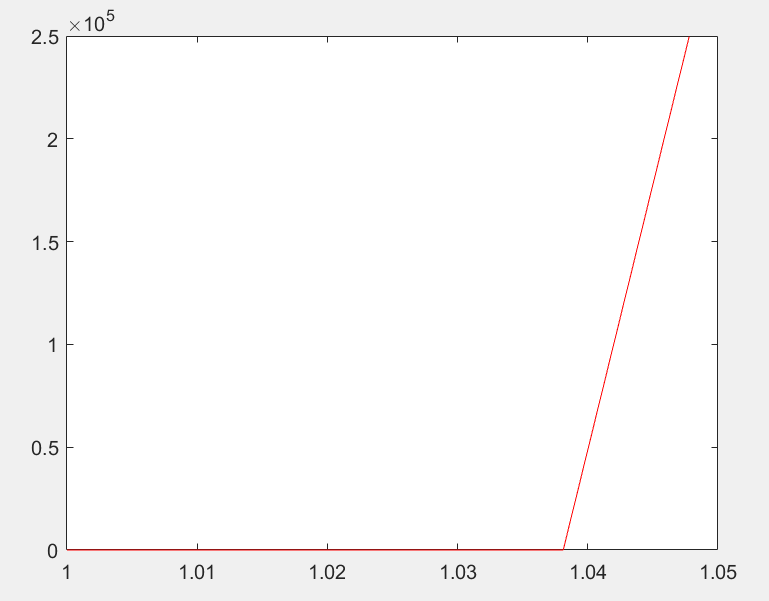
\includegraphics[width=5cm,height=5cm]{RKF54}
			
			\caption{问题1数值解的图像} \label{RKF54.label}
		\end{center}
	\end{figure}
	
	\begin{table}[H]
		\centering
		\begin{tabular}{|l|l|l|}
			\hline
			N & 误差 & 阶 \\ \hline
			8 & 0 & NaN \\ \hline
			16 & 0 & NaN \\ \hline
			32 & 0 & NaN \\ \hline
			64 & 0 & NaN \\ \hline
			128 & 0 & NaN \\ \hline
			256 & 0 & NaN \\ \hline
		\end{tabular}
	\end{table}
	
	
	
	\section{Discussion}
	对于第一个问题,由图像可以看出得到的数值解$y$的增长速率是很大的,因此采用两点线性插值得到的误差应该会是很大的。
	
	对于第二个问题,可以看到\text{Adams-Bashforth}公式的性能十分优良,得到的数值解甚至没有误差。


	\section{Computer Code}
	
	    \verbatiminput{RungeKutta.m}
	    \verbatiminput{RungeKutta5.m}
	    \verbatiminput{main.m}
	    \verbatiminput{main2.m}

\end{document}